\documentclass[12pt, letterpaper]{article}
\usepackage{graphicx} % LaTeX package to import graphics
\graphicspath{{images/}} % Configuring the graphicx package
\title{
    \underline{\textbf{Softcore System on a Chip Lab 1:}}
    \underline{\textbf{Rotating Square Circuit}} % Centered & underlined
   }
\author{David Edeni and Zach Martin}
\date{September 11th, 2025}
\begin{document}
\maketitle
\noindent \\\\\\\\ \underline{\textbf{Lab Description:}}
\maketitle \\\\This project implements a rotating square circuit on a four-digit seven-segment LED display. A square pattern is generated using segments (a, b, f, g) or (c, d, e, g). The circuit circulates the square around the four digits, with two control inputs: en (enable/pause) and cw (direction, cw = 1 means clockwise and cw = 0 means counterclockwise). The en input signal enables or pauses the circulation (en = 1 means the circuit is enabled/active and en = 0 means inactive) and the cw input signal specifies the direction of the circulation.\newpage
\noindent To implement our four-digit seven-segment LED rotating square circuit, we designed the following Block Diagram that produces a square pattern on the LED display at a rate visible to the human eye.\\\\\\
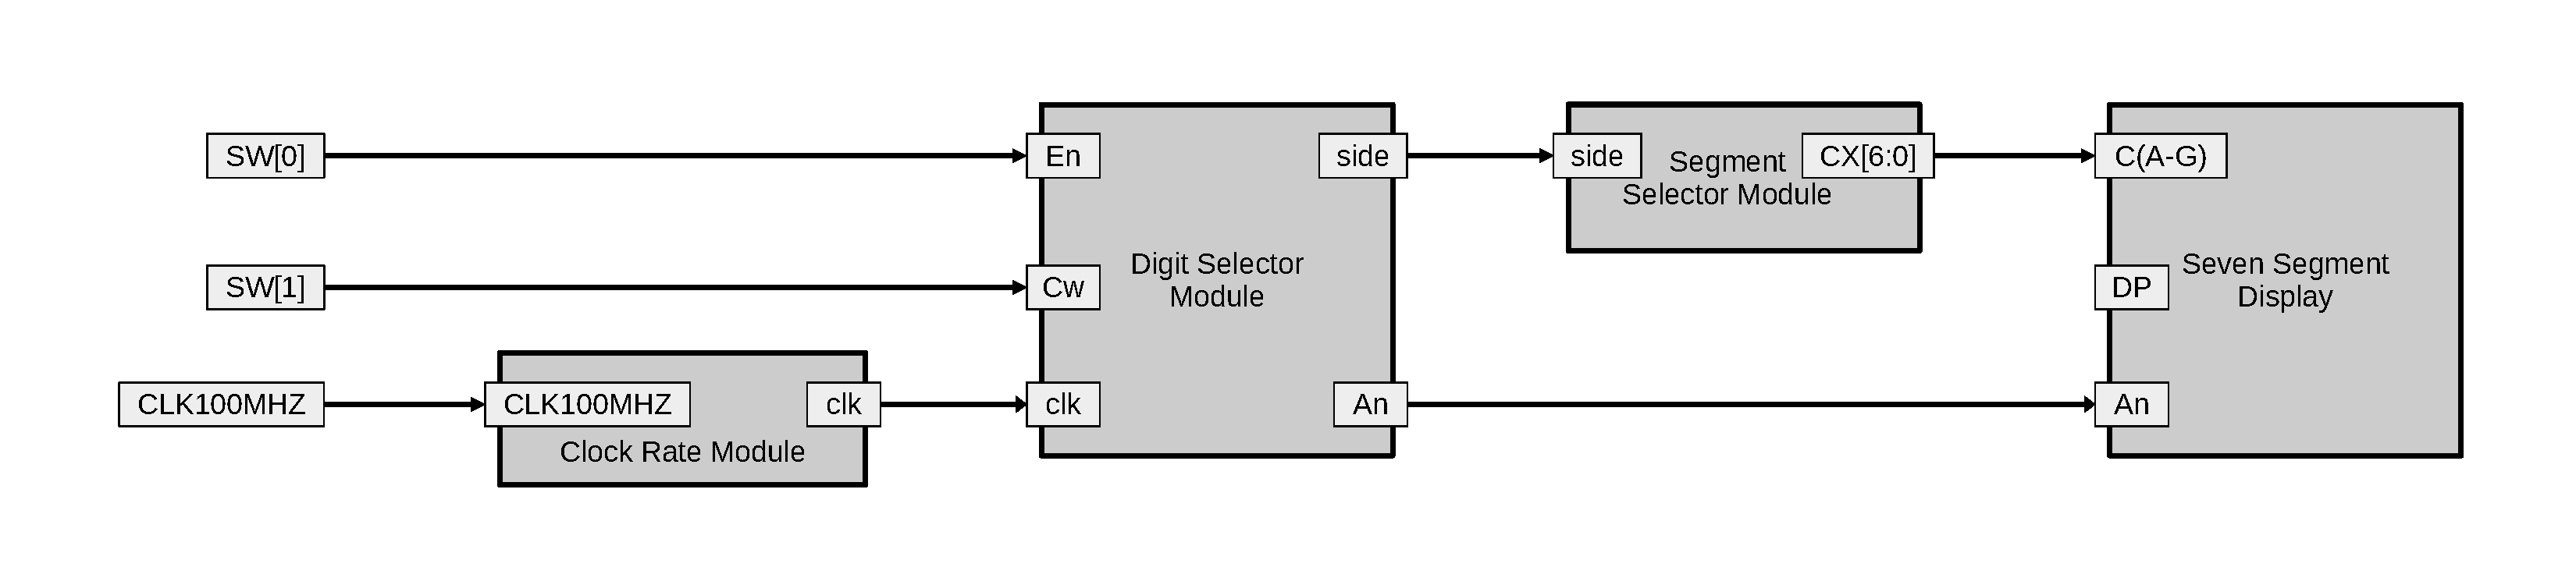
\includegraphics[width=1.2\textwidth]{SOC Project Rotating Square Circuit.pdf}
\\\\\\\\\\\\To implement this Block Diagram, we utilized four System Verilog Modules: digitSel.sv, segSel.sv, clockRate.sv, and top.sv.
\\\\\\\\\\The digitSel System Verilog module selects which digit of a four-digit seven-segment LED display should be active at a given time, and it rotates the active digit around the display in either a clockwise or counterclockwise direction based on the cw control signal. This module drives the digit enable (An) signal to control which of the four digits on the LED display lights up, while also generating a side signal that indicates which "half" of the rotation you are in.\newpage
\underline{Figure 1: The digitSel (digit selector) module:}\\\\\\
\includegraphics[width=0.55\textwidth]{digitSel.sv (digit selector) (top half) module.png}\\
\includegraphics[width=0.4\textwidth]{digitSel.sv (digit selector) (bottom half) module.png}\newpage
\noindent The segSel System Verilog module determines which segments (LED bars) of a seven-segment digit display should be lit up, depending on whether the "rotating square" is on the top side or bottom side of the display. This module selects whether the board's active digit shows the square's top or bottom half.\\\\\\
\underline{Figure 2: The segSel (segment selector) module:}\\\\\\
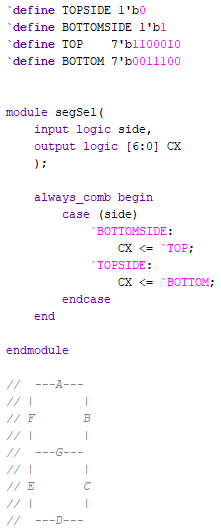
\includegraphics{segSel.sv (segment selector) module.png}
\\\\\\\\The clockRate System Verilog module is a clock divider / rate generator. The FPGA's main clock (100 MHz) is way too fast for human eyes, so to properly animaye the rotating square, you need a slower pulse ("tic"). This module divides the high-speed clock down to generate a visible slower timing signal.\\\\\\
\underline{Figure 3: The clockRate (segment selector) module:}\\\\\\
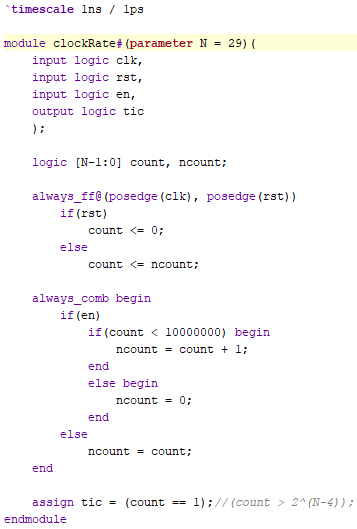
\includegraphics[width=0.6\textwidth]{clockRate.sv (counter) module.png}
\\\\Finally, the top System Verilog module is the glue that ties all our submodules (digitSel, segSel, clockRate) together to drive the rotating square circuit on the seven-segment display. This module connects the FPGA's hardware inputs (clock, switches) and outputs (seven-segment LEDs). It instantiates the three functional modules: digitSel, segSel, and clockRate, and wires them together so the square rotates across the 4-digit seven-segment display.\\\\\\
\underline{Figure 4: The top (square circuit implementation) module:}\\\\\\
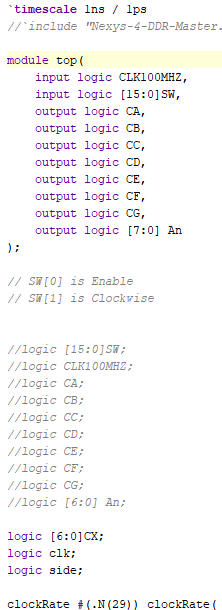
\includegraphics[width=0.3\textwidth]{top.sv module (top half).png}\\
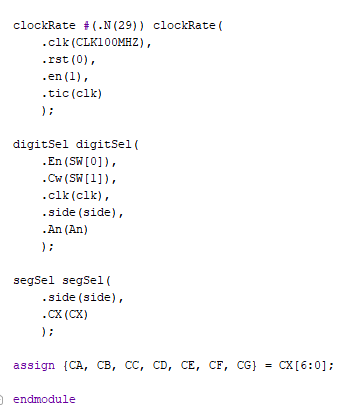
\includegraphics[width=0.45\textwidth]{top.sv module (bottom half).png}
\end{document}